\chapter{Struktura testa}

\section{Greške}

Nakon uvoda u osnovne pojmove vezane uz hipotezu pogledajmo s kolikom sigurnošću možemo tvrditi istinitost naše prosudbe u testu. Imamo 4 moguća ishoda testa:

% http://www.tablesgenerator.com/

\begin{table}[h]
\resizebox{\textwidth}{!}{%
\begin{tabular}{cc|c|c|}
\cline{3-4}
 &  & \multicolumn{2}{c|}{Nul hipoteza je} \\ \cline{3-4} 
 &  & Točna & Netočna \\ \hline
\multicolumn{1}{|c|}{\multirow{2}{*}{Presuda testa je:}} & Odbaci & \begin{tabular}[c]{@{}c@{}}Greška 1. vrste\\ Lažno pozitivni\\ $P = \alpha$\end{tabular} & Točno \\ \cline{2-4} 
\multicolumn{1}{|c|}{} & Prihvati & Točno & \begin{tabular}[c]{@{}c@{}}Greška 2. vrste\\ Lažno negativni \\ $P = \beta$\end{tabular} \\ \hline
\end{tabular}
}
\end{table}

Kakav god test odabrali da potvrdimo ili odbacimo $H_0$ on može rezultirati u greškama 1. ili 2. vrste. Evo jednog ilustrativnog primjera za grešku 1. vrste.

\subsection{Greške 1. vrste}

Odbacivanje nul hipoteze kada je ona točna naziva se greškom 1. vrste. \cite{engstat}. Radi daljnjeg pojašnjenja pogledati primjer u nastavku:

Situacija je sljedeća. Vi ste čuvar nekoga sela i vaša je dužnost oglasiti uzbunu ukoliko se vuk približava. Time je $H_0$ vuka nema. E ukoliko vuka stvarno nema, a vi ste oglasili uzbunu vi ste načinili pogrešku prve vrste ilitiga lažna pozitivnost.

Slični scenarij možete vidjeti i s testom za trudnoću. Ukoliko krećete od hipoteze  $H_0:$ \emph{Nema trudnoće} te $H_a:$ \emph{trudnoća} te stvarno niste trudni, ali test pokazuje trudnoću to je još jedan primjer greške 1. vrste. Njena vjerojatnost se označava grčkim slovom $\alpha$ te se naziva nivo značajnost testa \textit{(eng. significance level)}.

Pri samoj konstrukciji statističkog testa ukoliko je $H_0$ točna možemo lijepo uštimati $\alpha$ na prihvatljivu granicu te ga možemo lijepo uštimati jer često pretpostavljamo kako funkcija razdiobe izgleda.

\subsection{Greške 2. vrste}

No dobro, ovo je sve super, možemo podesiti test da nam je $\alpha \approx 0$ no sto time dobivamo? Tu u priču ulaze greške 2. vrste koje imaju vjerojatnost $\beta$. Ne odbacivanjem nul hipoteze, $H_0$, kada je ona netočna se naziva pogreška 2. vrste. \cite{engstat}

Koristeći primjere iz prethodne sekcije, vas test presudi da vuka nema dok on stvarno dolazi pred vaša vrata. Također vi ste trudni dok test za trudnoću to ne pokazuje dok nije prekasno. 

Vjerojatnost pojave greške 2. vrste označava se grčkim slovom $\beta$ te jepovezan s pojmom \emph{snaga testa} \textit{(eng. power)} koja iznosi $1-\beta$. Ona je definirana kao vjerojatnost da će test odbiti $H_0$ kada je ona lažna. 

Međutim $\beta$ je često nemoguće odrediti bez nekih pretpostavki. Npr. u testiranju očekivanja pretpostavljajući da je naša populaciju normalno distribuirama samo da se očekivanje razlikuje za neki $\delta$ tj. $\mu = \mu_0 + \delta$ uz $H_0: \; \mu = \mu_0$.

%Malo lijepse se izraziti oko "balansacije"
Kod izrade svakog statističkog testa dolazimo do biranja omjera snage i značajnosti istoga. Oni se ponašaju kao na klackalici, sto je veća snaga testa to je veća značajnost i obratno. Idealni test bi imao snagu 1 te značajnost 0, no to u praksi nije moguće, te time treba pažljivo odabrati ta dva parametra tijekom izrade samoga testa.

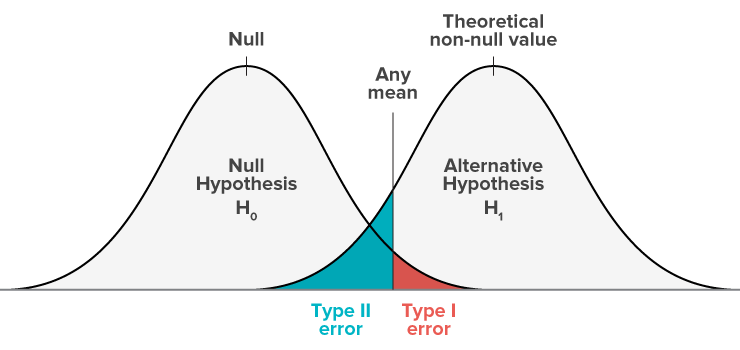
\includegraphics[width=\textwidth]{type12.png}

\section{P vrijednosti}
Sljedeći važan pojam u ovom kontekstu je p vrijednost. Ona se definira kao najmanja značajnost test, $\alpha$, za koju bi ovaj uzorak presudili odbacivanjem nul hipoteze, $H_0$ \cite{engstat}

Na slici \ref{fig:pvalue2} vidimo primjer. Neka je $H_0: \; \mu = 0$ te se uzima dvostrana alternativna hipoteza $H_a: \; \mu \ne 0$. Pretpostavlja se normalna distribucija s jediničnom varijancom.

Za opažanje iz uzorka $z = 1.96$ $p$ vrijednost našeg testa iznosi 0.05 sto znaci da za bilo koji $\alpha < 0.05$ presuda testa iznosi prihvaćanje nul hipoteze.

\begin{figure}[ph]
    \centering
    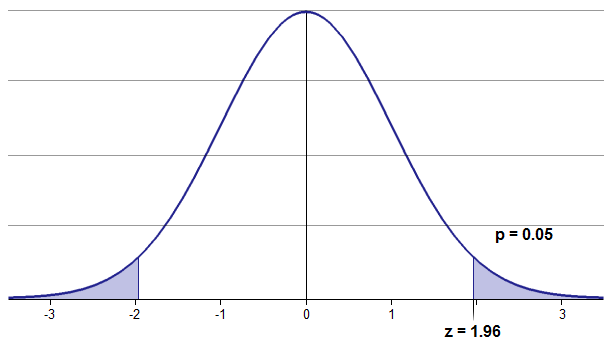
\includegraphics[width=\textwidth]{pvalue2.png}
    \caption{P vrijednost statistike $\mu = 0$ s distribucijom $X \sim \mathcal{N}(0,1)$}
	\label{fig:pvalue2}
\end{figure}


\section{Područje prihvaćanja}

Područje prihvaćanje \textit{eng. region of acceptance} se definira kao interval vrijednosti statistike uzorka za koji presuđujemo nul hipotezu, $H_0$. \cite{acceptance}

Ponovimo imamo $H_0$ hipotezu koja pretpostavlja neke parametre o distribuciju koju želimo testirati. \cite{vis3} 

Neka je slučajna varijabla $X \sim \mathcal{D}$.

Prvo definirajmo oznaku kao u većini literature:
$x_\alpha$ je $1-\alpha$ percentil te zadane distribucije. \cite{vis3} \cite{engstat} 

Za zadani nivo značajnosti $\alpha$ to zapravo znači  $P(x \in \left<l, u\right>) = 1-\alpha$. Tj. da šansa da ukoliko je $H_0$ točna, vjerojatnost točne presude iznosi $1-\alpha$

Najčešće se rabe tri tipa područja prihvaćanja:

\begin{itemize}
	\item Gornji: $x \in \left< x_\alpha, +\infty \right>$
	\item Dolni: $x \in \left<-\infty, x_{1-\alpha} \right>$
	\item Dvostrani: $x \in \left<x_{1-\frac{\alpha}{2}}, x_{\frac{\alpha}{2}} \right>$
\end{itemize}
